\documentclass{standalone}
\usepackage{tikz}
\usetikzlibrary{patterns, positioning}


\begin{document}
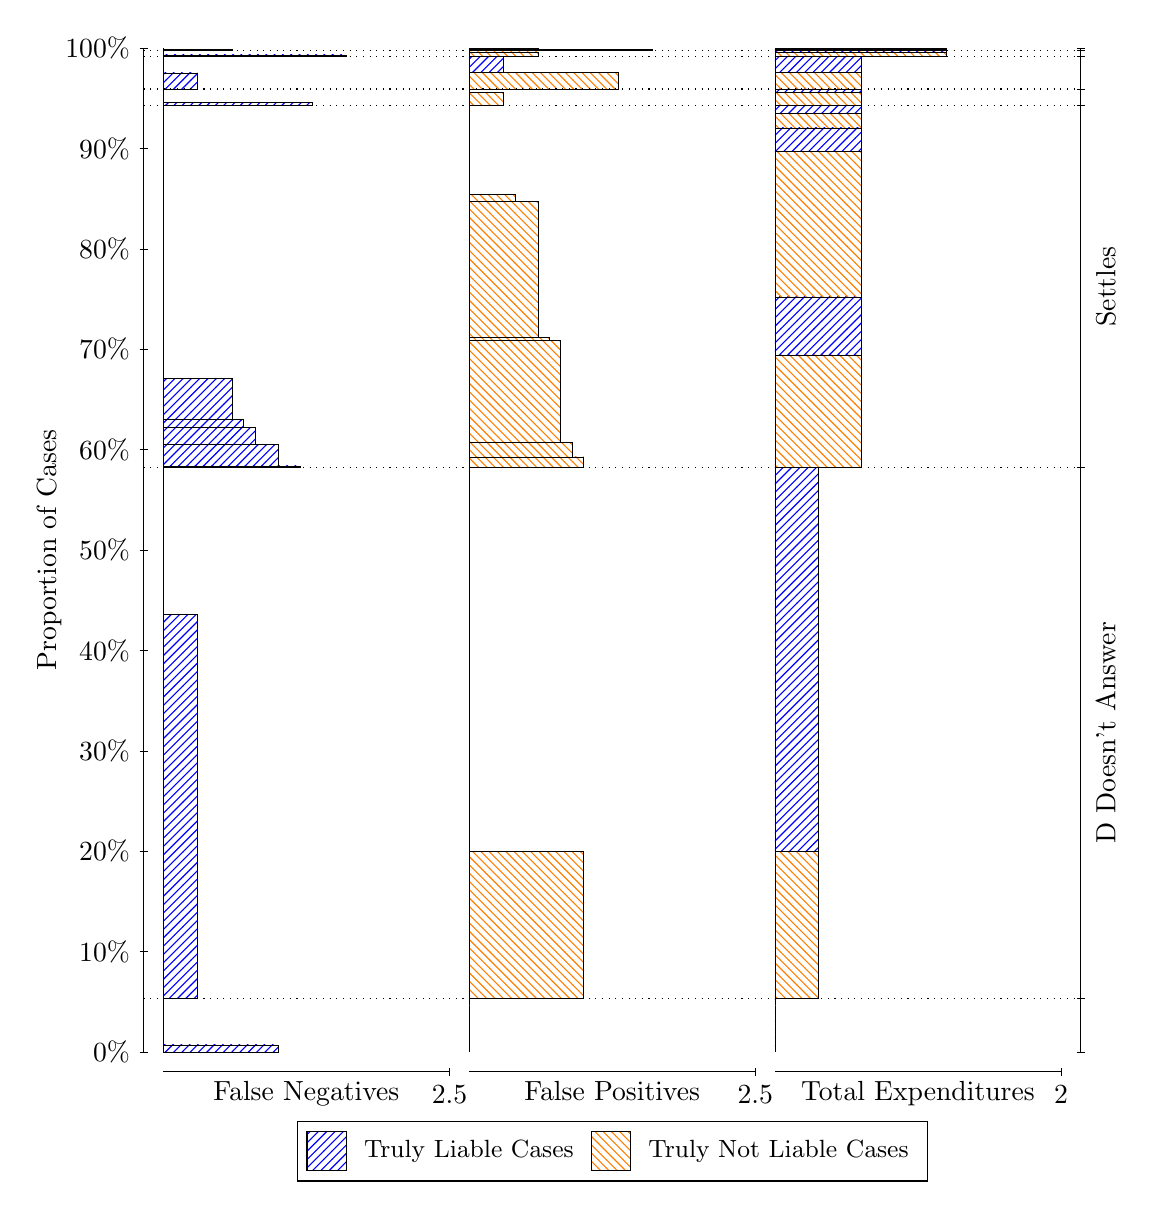
\begin{tikzpicture}
\draw[black, very thin] (1.5,1.75) -- (1.5,14.5);
\node[rotate=90, text=black, anchor=center] at (0.3, 8.125) {Proportion of Cases};
\draw[black, very thin] (1.45,1.75) -- (1.55,1.75);
\node[text=black, anchor=east] at (1.45, 1.75) {0\%};
\draw[black, very thin] (1.45,3.025) -- (1.55,3.025);
\node[text=black, anchor=east] at (1.45, 3.025) {10\%};
\draw[black, very thin] (1.45,4.3) -- (1.55,4.3);
\node[text=black, anchor=east] at (1.45, 4.3) {20\%};
\draw[black, very thin] (1.45,5.575) -- (1.55,5.575);
\node[text=black, anchor=east] at (1.45, 5.575) {30\%};
\draw[black, very thin] (1.45,6.85) -- (1.55,6.85);
\node[text=black, anchor=east] at (1.45, 6.85) {40\%};
\draw[black, very thin] (1.45,8.125) -- (1.55,8.125);
\node[text=black, anchor=east] at (1.45, 8.125) {50\%};
\draw[black, very thin] (1.45,9.4) -- (1.55,9.4);
\node[text=black, anchor=east] at (1.45, 9.4) {60\%};
\draw[black, very thin] (1.45,10.675) -- (1.55,10.675);
\node[text=black, anchor=east] at (1.45, 10.675) {70\%};
\draw[black, very thin] (1.45,11.95) -- (1.55,11.95);
\node[text=black, anchor=east] at (1.45, 11.95) {80\%};
\draw[black, very thin] (1.45,13.225) -- (1.55,13.225);
\node[text=black, anchor=east] at (1.45, 13.225) {90\%};
\draw[black, very thin] (1.45,14.5) -- (1.55,14.5);
\node[text=black, anchor=east] at (1.45, 14.5) {100\%};

\draw[black, very thin] (13.4,1.75) -- (13.4,14.5);
\draw[black, very thin] (13.35,1.75) -- (13.45,1.75);
\node[anchor=west] at (13.35, 1.75) {};
\draw[black, very thin] (13.35,2.4276) -- (13.45,2.4276);
\node[anchor=west] at (13.35, 2.4276) {};
\draw[black, very thin] (13.35,9.1782) -- (13.45,9.1782);
\node[anchor=west] at (13.35, 9.1782) {};
\draw[black, very thin] (13.35,13.769) -- (13.45,13.769);
\node[anchor=west] at (13.35, 13.769) {};
\draw[black, very thin] (13.35,13.98) -- (13.45,13.98);
\node[anchor=west] at (13.35, 13.98) {};
\draw[black, very thin] (13.35,14.398) -- (13.45,14.398);
\node[anchor=west] at (13.35, 14.398) {};
\draw[black, very thin] (13.35,14.467) -- (13.45,14.467);
\node[anchor=west] at (13.35, 14.467) {};
\draw[black, very thin] (13.35,14.5) -- (13.45,14.5);
\node[anchor=west] at (13.35, 14.5) {};

\draw[black, very thin, pattern color=blue, pattern=north east lines] (1.75,1.75) rectangle (3.2033,1.8402);
\draw[black, very thin, pattern color=orange, pattern=north west lines] (1.75,1.8402) rectangle (1.75,2.4276);
\draw[black, very thin, pattern color=blue, pattern=north east lines] (1.75,2.4276) rectangle (2.186,7.3036);
\draw[black, very thin, pattern color=orange, pattern=north west lines] (1.75,7.3036) rectangle (1.75,9.1782);
\draw[black, very thin, pattern color=blue, pattern=north east lines] (1.75,9.1782) rectangle (3.494,9.1921);
\draw[black, very thin, pattern color=blue, pattern=north east lines] (1.75,9.1921) rectangle (3.2033,9.4618);
\draw[black, very thin, pattern color=blue, pattern=north east lines] (1.75,9.4618) rectangle (3.058,9.4712);
\draw[black, very thin, pattern color=blue, pattern=north east lines] (1.75,9.4712) rectangle (2.9127,9.683);
\draw[black, very thin, pattern color=blue, pattern=north east lines] (1.75,9.683) rectangle (2.7673,9.7824);
\draw[black, very thin, pattern color=blue, pattern=north east lines] (1.75,9.7824) rectangle (2.622,10.307);
\draw[black, very thin, pattern color=orange, pattern=north west lines] (1.75,10.307) rectangle (1.75,13.769);
\draw[black, very thin, pattern color=blue, pattern=north east lines] (1.75,13.769) rectangle (3.6393,13.811);
\draw[black, very thin, pattern color=orange, pattern=north west lines] (1.75,13.811) rectangle (1.75,13.98);
\draw[black, very thin, pattern color=blue, pattern=north east lines] (1.75,13.98) rectangle (2.186,14.183);
\draw[black, very thin, pattern color=orange, pattern=north west lines] (1.75,14.183) rectangle (1.75,14.398);
\draw[black, very thin, pattern color=blue, pattern=north east lines] (1.75,14.398) rectangle (4.0753,14.414);
\draw[black, very thin, pattern color=orange, pattern=north west lines] (1.75,14.414) rectangle (1.75,14.467);
\draw[black, very thin, pattern color=blue, pattern=north east lines] (1.75,14.467) rectangle (2.622,14.484);
\draw[black, very thin, pattern color=orange, pattern=north west lines] (1.75,14.484) rectangle (1.75,14.5);
\draw[black, very thin, pattern color=orange, pattern=north west lines] (5.6333,1.75) rectangle (5.6333,2.3375);
\draw[black, very thin, pattern color=blue, pattern=north east lines] (5.6333,2.3375) rectangle (5.6333,2.4276);
\draw[black, very thin, pattern color=orange, pattern=north west lines] (5.6333,2.4276) rectangle (7.0867,4.3023);
\draw[black, very thin, pattern color=blue, pattern=north east lines] (5.6333,4.3023) rectangle (5.6333,9.1782);
\draw[black, very thin, pattern color=orange, pattern=north west lines] (5.6333,9.1782) rectangle (7.0867,9.3066);
\draw[black, very thin, pattern color=orange, pattern=north west lines] (5.6333,9.3066) rectangle (6.9413,9.4907);
\draw[black, very thin, pattern color=orange, pattern=north west lines] (5.6333,9.4907) rectangle (6.796,10.787);
\draw[black, very thin, pattern color=orange, pattern=north west lines] (5.6333,10.787) rectangle (6.6507,10.821);
\draw[black, very thin, pattern color=orange, pattern=north west lines] (5.6333,10.821) rectangle (6.5053,12.553);
\draw[black, very thin, pattern color=orange, pattern=north west lines] (5.6333,12.553) rectangle (6.2147,12.64);
\draw[black, very thin, pattern color=blue, pattern=north east lines] (5.6333,12.64) rectangle (5.6333,13.769);
\draw[black, very thin, pattern color=orange, pattern=north west lines] (5.6333,13.769) rectangle (6.0693,13.937);
\draw[black, very thin, pattern color=blue, pattern=north east lines] (5.6333,13.937) rectangle (5.6333,13.98);
\draw[black, very thin, pattern color=orange, pattern=north west lines] (5.6333,13.98) rectangle (7.5227,14.195);
\draw[black, very thin, pattern color=blue, pattern=north east lines] (5.6333,14.195) rectangle (6.0693,14.398);
\draw[black, very thin, pattern color=orange, pattern=north west lines] (5.6333,14.398) rectangle (6.5053,14.451);
\draw[black, very thin, pattern color=blue, pattern=north east lines] (5.6333,14.451) rectangle (5.6333,14.467);
\draw[black, very thin, pattern color=orange, pattern=north west lines] (5.6333,14.467) rectangle (7.9587,14.482);
\draw[black, very thin, pattern color=blue, pattern=north east lines] (5.6333,14.482) rectangle (6.5053,14.5);
\draw[black, very thin, pattern color=orange, pattern=north west lines] (9.5167,1.75) rectangle (9.5167,2.3375);
\draw[black, very thin, pattern color=blue, pattern=north east lines] (9.5167,2.3375) rectangle (9.5167,2.4276);
\draw[black, very thin, pattern color=orange, pattern=north west lines] (9.5167,2.4276) rectangle (10.062,4.3023);
\draw[black, very thin, pattern color=blue, pattern=north east lines] (9.5167,4.3023) rectangle (10.062,9.1782);
\draw[black, very thin, pattern color=orange, pattern=north west lines] (9.5167,9.1782) rectangle (10.607,10.603);
\draw[black, very thin, pattern color=blue, pattern=north east lines] (9.5167,10.603) rectangle (10.607,11.339);
\draw[black, very thin, pattern color=orange, pattern=north west lines] (9.5167,11.339) rectangle (10.607,13.192);
\draw[black, very thin, pattern color=blue, pattern=north east lines] (9.5167,13.192) rectangle (10.607,13.485);
\draw[black, very thin, pattern color=orange, pattern=north west lines] (9.5167,13.485) rectangle (10.607,13.669);
\draw[black, very thin, pattern color=blue, pattern=north east lines] (9.5167,13.669) rectangle (10.607,13.769);
\draw[black, very thin, pattern color=orange, pattern=north west lines] (9.5167,13.769) rectangle (10.607,13.937);
\draw[black, very thin, pattern color=blue, pattern=north east lines] (9.5167,13.937) rectangle (10.607,13.98);
\draw[black, very thin, pattern color=orange, pattern=north west lines] (9.5167,13.98) rectangle (10.607,14.195);
\draw[black, very thin, pattern color=blue, pattern=north east lines] (9.5167,14.195) rectangle (10.607,14.398);
\draw[black, very thin, pattern color=orange, pattern=north west lines] (9.5167,14.398) rectangle (11.697,14.451);
\draw[black, very thin, pattern color=blue, pattern=north east lines] (9.5167,14.451) rectangle (11.697,14.467);
\draw[black, very thin, pattern color=orange, pattern=north west lines] (9.5167,14.467) rectangle (11.697,14.482);
\draw[black, very thin, pattern color=blue, pattern=north east lines] (9.5167,14.482) rectangle (11.697,14.5);
\draw[black, dotted] (1.5,2.4276) -- (13.4,2.4276);
\draw[black, dotted] (1.5,9.1782) -- (13.4,9.1782);
\draw[black, dotted] (1.5,13.769) -- (13.4,13.769);
\draw[black, dotted] (1.5,13.98) -- (13.4,13.98);
\draw[black, dotted] (1.5,14.398) -- (13.4,14.398);
\draw[black, dotted] (1.5,14.467) -- (13.4,14.467);
\draw[black, very thin] (1.75,1.5) -- (5.3833,1.5);
\node[text=black, anchor=north] at (3.5667, 1.5) {False Negatives};
\draw[black, very thin] (5.3833,1.45) -- (5.3833,1.55);
\node[text=black, anchor=north] at (5.3833, 1.45) {2.5};

\draw[black, very thin] (5.6333,1.5) -- (9.2667,1.5);
\node[text=black, anchor=north] at (7.45, 1.5) {False Positives};
\draw[black, very thin] (9.2667,1.45) -- (9.2667,1.55);
\node[text=black, anchor=north] at (9.2667, 1.45) {2.5};

\draw[black, very thin] (9.5167,1.5) -- (13.15,1.5);
\node[text=black, anchor=north] at (11.333, 1.5) {Total Expenditures};
\draw[black, very thin] (13.15,1.45) -- (13.15,1.55);
\node[text=black, anchor=north] at (13.15, 1.45) {2};


\node[text=black, centered, rotate=90] at (13.72, 5.8029) {D Doesn't Answer};
\node[text=black, centered, rotate=90] at (13.72, 11.473) {Settles};





\draw (7.449999999999999,1.5) node[draw=none] (baseCoordinate) {};
\begin{scope}[align=center]
        \matrix[scale=0.5, draw=black, below=0.5cm of baseCoordinate, nodes={draw}, column sep=0.1cm]{
            \node[rectangle, draw, minimum width=0.5cm, minimum height=0.5cm, pattern color=blue, pattern=north east lines] {}; &
            \node[draw=none, font=\small, text=black] (B) {Truly Liable Cases}; &
            \node[rectangle, draw, minimum width=0.5cm, minimum height=0.5cm, pattern color=orange, pattern=north west lines] {}; &
            \node[draw=none, font=\small, text=black] (B) {Truly Not Liable Cases}; \\
            };
\end{scope}

\end{tikzpicture}
\end{document}